\chapter{The cultural, sociolinguistic and typological context}\label{chap:1}
\section{Introduction}\label{sec:introduction-1}

\is{purpose of the grammar|(}Kagayanen (ISO 639-3 CGC) is a Western Austronesian language spoken by approximately 30,000 individuals\is{population} in the Central Philippines. This work is a descriptive grammar, following a general typologically-oriented framework similar to “\isi{Basic Linguistic Theory}” as described by \citet{dixon2010a, dixon2010b}. We believe that a typological framework based on prose description rather than complex formalisms is most appropriate for describing the unique and remarkable features of Kagayanen, without imposing presuppositions of universality inherent in many form-oriented approaches. The fundamental presupposition of our approach is simply that any language is a symbolic system used by human beings for communication. From this it follows that the forms of any language can best be described and understood in terms of the common human need to communicate. Therefore, considerations of semantics (meaning) and pragmatics (usage) underlie all discussion and explanation of structural patterns.

This work is primarily synchronic in that it describes the state of Kagayanen grammar at a particular “slice” in time between about 1987 and 2023. While there is significant variation in the speech of individual communities even within this relatively brief historical period, we attempt to describe common patterns in the major communities, as described below. Dialect variation and historical considerations will be mentioned at various points, but the synchronic description of the common spoken language will remain at the forefront.\is{purpose of the grammar|)}

\section{The Kagayanen people and language}\label{sec:1.2} \label{sec:peopleandlanguage}
\subsection{Language name and classification}\label{sec:1.2.1} \label{sec:languagenameandclassification}

\is{names of the language|(}There are at least four names and spellings used for the language described in this grammar. \citet{dyen1965} called it Cagayanon, \citet{llamzon1974} called it Cagayancillo, \citet{elkins1974} called it Cagayano. \citet{zorc1977} was the first to call it Kagayanen. \citet{harmon1977} also called it Kagayanen, both because of the precedent set by Zorc, and because this is the standard spelling of the term speakers commonly use to refer to their own language (IPA [kagaˈjanɤ̞n]).  However, some Kagayanen speakers refer to themselves as Cagayano and to their language as Kagayanen. Other names some people use are Kagay-anen and Kinagayanen.\is{names of the language|)}

\is{genetic affiliation|(}
The Kagayanen language is classified in the Ethnologue \citep{eberhard2023} as Austronesian, Malayo-Polynesian, Philippine, Greater Central Philippine, Manobo, North. However, there has been considerable controversy about its classification over the years. The following is a summary of \citegen{harmon1977} discussion of the classification of the Kagayanen language.

\citet{dyen1965} classified Kagayanen as a member of the “Tagalic Hesion” within the Bisayan Cluster, parallel to \isi{Tagalog}, and \isi{Mamanwa}, using lexicostatistics alone.  According to \citet[639]{elkins1974}, Dyen later came to a different understanding and decided that Kagayanen was a Manobo language rather than a Tagalic language. \citet{elkins1974} went on to classify Kagayanen as a member of the Manobo group based on a more inclusive comparative study. In particular, Elkins found that Kagayanen possesses seven of fifteen Manobo lexical innovations, and all of the pronoun innovations exclusive to the Manobo languages. \citet{llamzon1974} suggested that Kagayanen was closest to languages spoken in Palawan, particularly Tagbanwa Kalamian, based on only one innovation -- the use of the prenominal particle \textit{ta} as a common noun possessive marker. 

We agree with \citet{elkins1974} and \citet{harmon1977} that the evidence is stronger for a Manobo rather than a Palawanic or Bisayan heritage. Furthermore, the high proportion of lexical similarity with Bisayan languages is undoubtedly due to borrowing facilitated by geographic proximity as well as economic and sociolinguistic pressure from Bisayan languages such as \isi{Hiligaynon} and \isi{Kinaray-a} (see \sectref{sec:1.3} below). The deeper comparative evidence provided by \citet{elkins1974} clearly indicates a Manobo connection. \figref{fig:kagayanenfamilytree} illustrates the relevant portions of the Greater Central Philippine language group \citep{blust1991} according to contemporary understandings, with both Llamzon's and Elkins' hypothesized positions of Kagayanen indicated.

% \begin{figure}
%     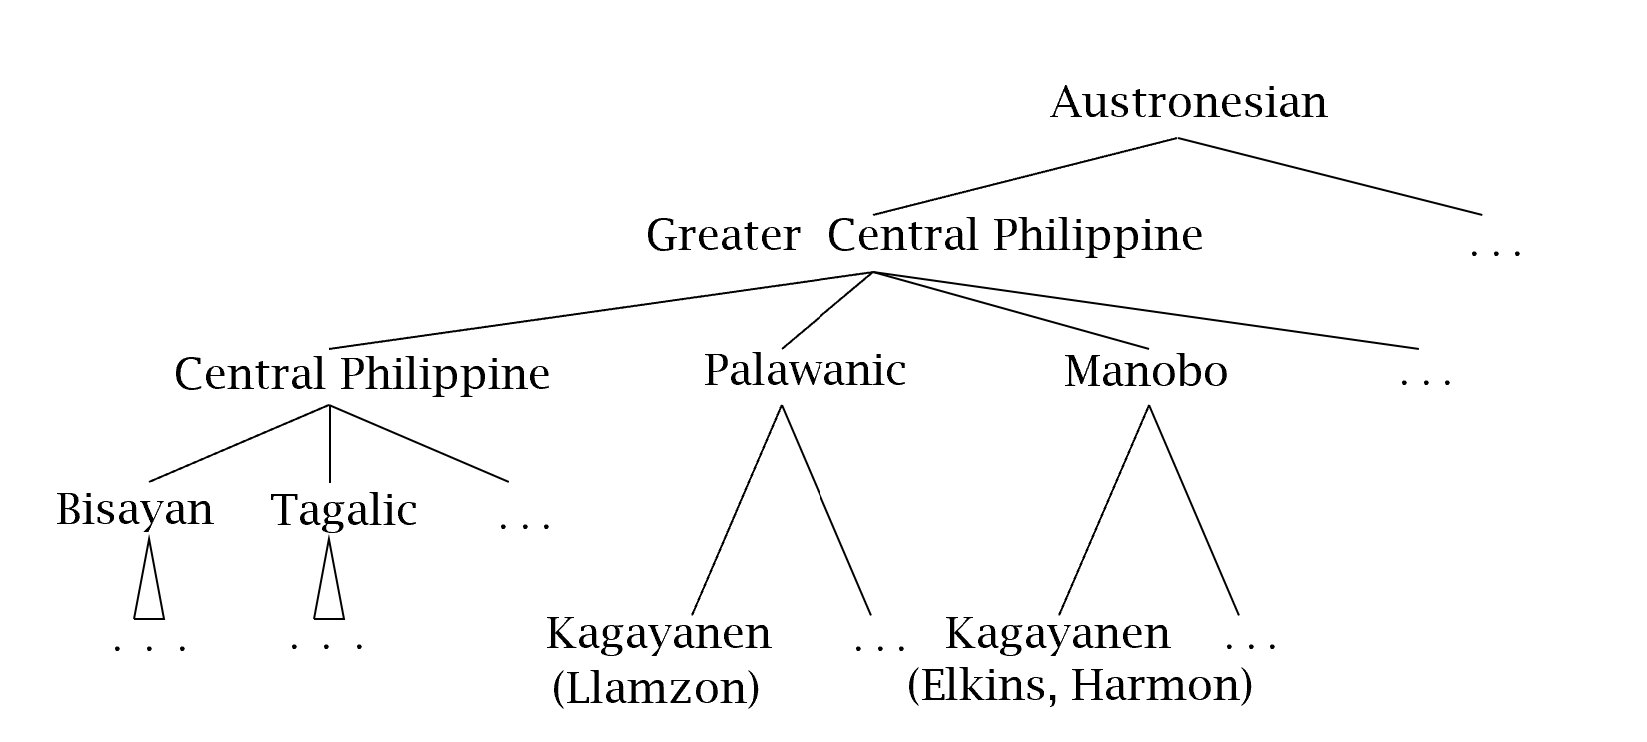
\includegraphics[scale=0.55]{figures/Kagayanen_family_tree.png}
%     \caption{Two possible positions of Kagayanen in the Austronesian family}
%     \label{fig:kagayanenfamilytree}
% \end{figure}

\begin{figure}
\begin{forest}
[Austronesian
    [Greater Central Philippine
        [Central Philippine
            [Bisayan
                [...,roof]
            ]
            [Tagalic
                [...,roof]
            ]
            [...]
        ]
        [Palawanic
            [Kagayanen\\(Llamzon)]
            [...]
        ]
        [Manobo
            [Kagayanen\\(Elkins{,} Harmon)]
            [...]
        ]
        [...]
    ]
    [...]
]
\end{forest}
\caption{Two possible positions of Kagayanen in the Greater Central Philippine group of languages}
\label{fig:kagayanenfamilytree}
\end{figure}

Most of the languages in the Manobo group are located on Mindanao and Camiguin Island in the southern Philippines, while Kagayanen is located in the central part of the country. If Kagayanen really is in the Manobo group, then it is by far the furthest north of the group. The geographically closest neighboring languages are Agutaynen and \isi{Cuyonon} to the North and \isi{Kinaray-a} and \isi{Hiligaynon} to the east on Panay island. These languages, according to \citet{zorc1977} and \citet{harmon1977}, are Bisayan. This observation is uncontroversial at the present state of scholarship. In any case, Kagayanen has a higher percentage of typically Bisayan words than other languages in the Manobo group. \citet[21--22]{harmon1977} states that this fact could mean one of three things: 1) Kagayanen, Bisayan languages and Manobo languages are three branches of a proto-Bisayan-Manobo group, 2) Kagayanen is a Bisayan language, 3) Kagayanen is a Manobo language whose speakers migrated from an original Mindanao homeland to the Cagayan islands and subsequently borrowed many words from the languages of the people with whom they traded. Our opinion, as outlined above, coincides with Harmon's third possibility, that Kagayanen is a Manobo language having many grammatical characteristics of Manobo languages with heavy lexical influence from Bisayan.\is{genetic affiliation|)}

\subsection{Demography and history}\label{sec:1.2.2} \label{sec:demographyandhistory}
\is{demography|(}

The 2007 Philippine census indicates that 42,000 people identify themselves as Kagayanen, including approximately 30,000 speakers who use the language in daily life. At that time, there were 6,000 Kagayanens in the Cagayan Islands, 6,000 in Puerto Princesa City, which is the capital of Palawan Province, 18,000 in Roxas in northern Palawan and 12,000 in Narra in southern Palawan. There are Kagayanens also living in other parts of the Philippines and abroad.

The origin of the people living in the Cagayan Islands (Municipality of Cagayancillo) is uncertain. In 1975 Carol Harmon interviewed second and third generation Kagayanens in Puerto Princesa (Palawan) and in Cagayancillo concerning their ethnic origins \citep[4--5]{harmon1977}. Some said their parents or grandparents had come from Panay Island where \isi{Kinaray-a} is spoken, and learned to speak Kagayanen, the language of the people who already inhabited Cagayancillo. Others said that they and their families had always lived in the Cagayan Islands as far as they knew, and that they had no knowledge of an earlier home. If \isi{Kinaray-a} was spoken as a first language by people who migrated to the Cagayan Islands, this could explain why Kagayanen vocabulary contains so many Bisayan words.

One theory of the origin of the original Kagayanen language is that a group of Manobo speakers migrated up through the Visayas, borrowing Bisayan words as they went, and finally settled in the Cagayan Islands. As Bisayan people later migrated to the Cagayan Islands and intermarried with the people there, the language spoken in the Cagayan Islands incorporated additional Bisayan words. In addition, the people in the Cagayan Islands traded with Bisayan people in nearby seaports on Panay and Negros islands, thus resulting in more borrowing of Bisayan words.

Another theory, suggested by a Kagayanen shaman in personal communication, is that the original inhabitants of the Cagayan Islands migrated from Cagayan de Sulu, in the extreme south of the country. Then Bisayan people from Panay and Negros migrated to the Cagayan Islands and intermarried. This theory would explain why some words in languages in the area of western Mindanao and Tawi-Tawi in the Southwest are cognate with words in Kagayanen.

A third theory, derived from personal conversations with Kagayanen speakers and from oral texts, is that the people living on the Cagayan Islands originated from Busuanga, Coron area, where speakers call themselves Calamianes Kagayanen. The language of that area indeed shares many similarities with Kagayanen as described in this grammar.

In the early 1950s, many people on Cagayancillo began migrating to mainland Palawan and to other places in the Philippines forming small communities wherever they settled. Today Kagayanens continue to migrate to larger cities such as Manila, Iloilo, Puerto Princesa City, Cebu, and Davao in search of education and employment opportunities.

\subsection{Geography}\label{sec:1.2.3}

The ethnocenter of the Kagayanen language group is the Cagayan Islands, a group of 31 islands and islets located in the Sulu Sea about 178 nautical miles east of the provincial capital city, Puerto Princesa, on the island of Palawan and 72 nautical miles west of Silay City, Negros Oriental. It is located at 9° 34′ 60″ N. latitude and 121° 12′ E. longitude (see \figref{fig:locationofkagayanencommunities}).

\begin{figure}
    \centering
    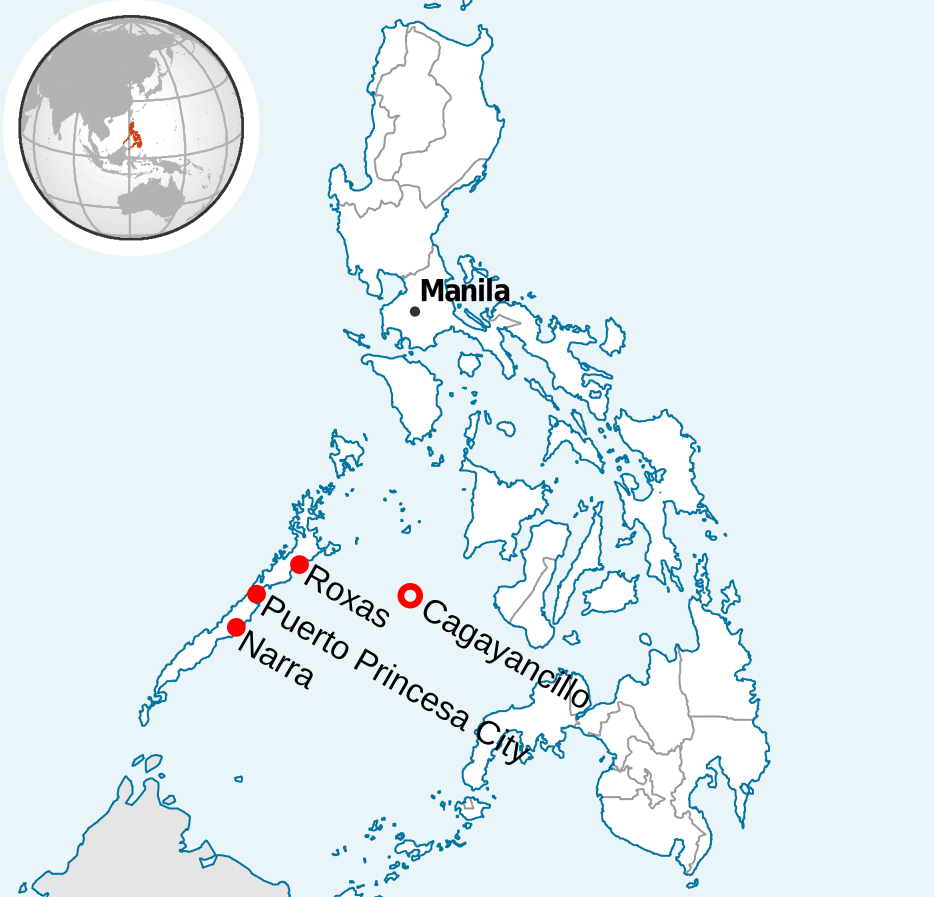
\includegraphics{figures/map_Palawan.png}
    \caption{Locations of key Kagayanen communities}
    \label{fig:locationofkagayanencommunities}
\end{figure}
Although the Cagayan Islands are the ethnocenter, communities of Kagayanen speakers are scattered throughout Palawan Province. The largest concentrations are on the island of Palawan in Roxas (not to be confused with Roxas City on the island of Panay), Narra and Puerto Princesa cities. Smaller clusters live in the mun icipality of Coron, the north Palawan region of Busuanga, the southern island of Balabac, and in the Western Visayas including the provinces of Iloilo, Antique, and Negros Occidental, as well as the national capital, Manila. 

\subsection{Economic activity}\label{sec:1.2.4} \label{sec:economicactivity}
\is{culture|(} \is{economic activity|(}

Kagayanens are a lowland culture. They are mostly agri- and aquaculturists. They grow crops of cassava, corn, sorghum and various kinds of vegetables and fruit for their personal consumption. They fish and harvest sea crops for their own families and occasionally for sale on a small scale. Today, many Kagayanens are college graduates and have become businesspersons and professionals.
\is{economic activity|)}
\is{culture|)}
\is{demography|)}
\section{Sociolinguistic situation}\label{sec:1.3} \label{sec:sociolinguisticsituation}
\is{status of Kagayanen|(}

As in many parts of the Philippines, Palawan is a “melting pot” of languages due to heavy migrations from other parts of the country. The Ethnologue \citep{eberhard2023} indicates that there are few monolingual speakers of Kagayanen, since inhabitants of the Cagayan Islands also need to speak languages such as \isi{Hiligaynon}, \isi{Kinaray-a}, \isi{Cebuano}, \isi{Tagalog} and \isi{Cuyonon}. In fact, most Kagayanens are multilingual to varying degrees in at least three of these languages, as well as in English. 

Since Palawan is so linguistically diverse, \isi{Filipino} (the Tagalog-based National Language) is the lingua franca on mainland Palawan and the second language of Kagayanens living there. Kagayanen spoken on mainland Palawan is heavily influenced by \isi{Filipino}. Some Kagayanen parents on mainland Palawan and other places in the Philippines tend to teach their children to speak \isi{Filipino} even within the home. This indicates the beginning of the process of a shift to \isi{Filipino}.

However, Cagayancillo (the official municipality corresponding to the Cagayan Islands) is linguistically far more homogeneous. \isi{Hiligaynon} influences the language in Cagayancillo more than on mainland Palawan, since Kagayanen speakers relate more to the Visayas for trade and educational opportunities. Furthermore, beginning in the 1600s under Spanish rule, until 1935 the Cagayan Islands were under the jurisdiction of Antique Province (on Panay in the Visayas). \isi{Hiligaynon} (Ilongo) is the second language of older Kagayanens living in Cagayancillo, and therefore words tend to be borrowed from \isi{Hiligaynon} rather than \isi{Filipino}. Another respect in which the language situation in Cagayancillo is distinct is that children speak Kagayanen in their homes. This tends not to be the case in Kagayanen communities in other parts of the Philippines.

In Cagayancillo, Kagayanen is used in all domains, in local administrative affairs, in commerce and religion. In the 2013 school  year, the department of Education launched a \isi{multilingual education} program on Cagayancillo which began to use Kagayanen as the medium of instruction in grades 1--3. While in the past letters were written either in \isi{Hiligaynon} or \isi{Tagalog}, today the tendency is to write letters in Kagayanen. On mainland Palawan, \isi{Filipino} is considered appropriate for school, market, church and reading. Among Kagayanen first-language speakers in all locations, we estimate that the adult \isi{literacy rate} is about 95\%. 

It should be noted that, because of the high degree of multilingualism and intercultural interaction in Kagayanen communities, \isi{code mixing} is a common feature of everyday conversation. We have footnoted some particularly clear and significant instances of code mixing in the conversational and corpus examples appearing in this grammar. However, we have refrained from noting every instance of code mixing for two reasons: 1) Sometimes it is not clear whether a particular usage is code mixing or not, and 2) noting every single instance would unnecessarily clutter the text with footnotes. 
\is{status of Kagayanen|)}

\section{Data sources}\label{sec:1.4} \label{sec:datasources}
\is{data base|(}
\largerpage

The corpus on which the current study is based consists of two broad data types: 1) verified elicited or conversational data, and 2) texts. Insofar as possible, examples in this work come from texts. Elicited or conversational data fill in gaps that are not attested in the text corpus, and are used to illustrate the range of possibilities for syntactic constructions that are rare in the texts. When text examples are complex and difficult to follow, a concise elicited example will often adequately serve the purpose. In many cases, elicited examples are based on examples from the texts. All elicited examples have been verified by two or more speakers.

The texts on which this description is based were gathered over a period of 21 years, during which Carol Pebley lived for four years in Cagayancillo, Palawan, the homeland of the Kagayanen people, and about 18 years in Kagayanen communities in Manila and in Puerto Princesa City, the provincial capital of Palawan province (see map, \figref{fig:locationofkagayanencommunities}).

The text material consists of 365 texts totaling 149,350 words. Of these, there are 116 oral texts of 59,036 words in total and 249 written texts with 90,314 words. The texts were gathered in various ways by Carol Pebley, \name{Jacqueline}{Huggins}, and \name{Louise}{MacGregor}. Some were elicited orally, recorded and transcribed. Others were elicited as written texts. Some were recorded public speeches at special occasions such as graduations, Foundation Day celebrations and sermons. Some came from a writing contest and a writer’s workshop held on Cagayancillo, coordinated by Louise MacGregor and \name{Lillian}{Underwood} in 1988. Some written texts came from personal correspondence. The written texts and the transcriptions of the oral texts were incorporated into a digital database.

Each text in the database has a unique reference code with this format (L refers to letters, and N refers to numbers):
\TabPositions{2cm,4cm,6cm,8cm}
\begin{itemize}
\item[] L\textsubscript{1} L\textsubscript{2} L\textsubscript{3} L\textsubscript{4} -- L\textsubscript{5} -- NN

\item[] L\textsubscript{1} L\textsubscript{2} = Two-letter code identifying the author of the text.

\item[] L\textsubscript{3} = O (oral) or W (written)

\item[] L\textsubscript{4} = Genre (N for narrative, E for expository, P for procedural, O for poetry, L for letter, R for riddle, I for interview, B for behavioral, C for dialogue or conversation, and V for proverb)

\item[] L\textsubscript{5} = Linguist (C for Carol Pebley, J for \name{Jacqueline}{Huggins}, L for \name{Louise}{MacGregor}, and T for the team.)

\item[] NN = the text number.
\end{itemize}

For example, the identifier “DBON-C-02” would mean that the text was an oral narrative composed by \name{Darlie}{Bundal}, recorded and transcribed by Carol Pebley, and is the second text contributed by this author.
\appref{app:a} summarizes the content of the text corpus by genre, 4-letter code and number of texts and words.

Elicited data come from the extensive field notes of Carol Pebley, \name{Jacqueline}{Huggins}, and \name{Louise}{MacGregor}. Whenever a conversational or elicited example is used in this grammar, no reference is provided following the free translation. In every case, such examples have been verified by at least two mother-tongue speakers. 

A dictionary has been in process since the beginning of the project in 1974 when Scott\ia{MacGregor, Scott} and \name{Louise}{MacGregor} lived and worked in Caguisan, Narra, Palawan, a Kagayanen community on mainland Palawan. Since Jacqueline and Carol joined the project in 1986 and lived on the home island in Cagayancillo, they collected additional words absent in the MacGregor dictionary, which were subsequently merged with the MacGregor dictionary, resulting in a team dictionary with approximately 7,000 entries and thousands of example sentences illustrating different combinations of verbal affixation in context. Work on Kagayanen lexicography is ongoing. A dictionary for linguists is being prepared by \name{Louise}{MacGregor}, and another for Kagayanen speakers is being prepared by \name{Jacqueline}{Huggins}.\is{data base|)}

\section{Previous research}\label{sec:1.5} \label{sec:previousresearch}
\is{literature, previous|(}\is{research, previous|(}

In this section we will report on previous linguistic research on Kagayanen and the most closely related language, Binukid. Several have written about the classification of the language, as discussed in \sectref{sec:1.2.1} above. Louise MacGregor \citep{macgregor1995} contributed an introduction to Kagayanen and a wordlist to the Comparative Austronesian Dictionary edited by Darrell T. Tryon \citep{tryon1995}. \citet{macgregor1999} consists of two interlinearized texts. \citet{pebley1998} describes the prefix \textit{m}- in Kagayanen and how its use is connected with intransitivity and causation or volition. \citet{pebleyfunctions1999} describe the functions of fronted noun phrases. \citet{pebleysketch1999} provides a sketch of Kagayanen clause structure. \citet{pebleyparticipant1999} describes the participant reference system, and \citet{pebleyenclitic1999} describes the discourse function of the three demonstrative determiners \textit{i}, \textit{an} and \textit{ya}.
\citet{olson2010} describe the articulation of the interdental approximate, and the acoustic properties of the vowel space. \citet{olson2007a} and \citet{olson2008} describe the acoustic and articulatory properties of the interdental approximate in Kagayanen. These materials and more can be accessed via Glottolog at \url{https://glottolog.org/resource/languoid/id/kaga1256}.

\is{Binukid|(}Much has been written on Binukid, the language most closely related to Kagayanen. William \citet{atherton1953} describes the phonemes, and in addition has several unpublished works, including grammar notes, a description of the personal pronouns  and verb morphology. Kathleen \citet{meiklejohn1953} also describe the phonemes. Theodoro \citet{llamzon1974} includes a section on Binukid describing the genetic classification, culture, phonemes, pronouns and verb morphology. Adam Peng and Loren Billings \citep{peng2006} describe the pronominal system.  Ursula \citet{post1965c} describes morphophonemic alternations. \citet{postsentence1968} describes sentence structure, \citet{postphrase1968} phrase and clause structure, \citet{post1978} Binukid texts, and \citet{posttagmemes1965} describes personal pronouns. \citet{reid1971} consists of a wordlist and phonology. \name{Mary Jane}{Gardner} and \name{Ursula}{Post} compiled a dictionary of Binukid including a brief sketch of the phonology and grammar. This work was edited and published by Fe Otanes and Hazel Wrigglesworth \citep{otanes1992}. Donald \citet{stark1961} reconstructed a proto-language with reflexes in Binukid and Dibabaon-Mandayan. The website of SIL Philippines includes several downloadable files and papers concerning Binukid, including the Gardner and Post dictionary. The World Atlas of Linguistic Structures (WALS) includes a page listing all resources relevant to Binukid (see \url{https://wals.info/languoid/lect/wals_code_bkd}). As of 2024, no comprehensive grammatical description of Kagayanen or Binukid exists.\is{Binukid|)}
\is{research, previous|)}
\is{literature, previous|)}

\section{Typological sketch}\label{sec:1.6} \label{sec:typology}
\is{typology|(}
\subsection{Morphological typology}\label{sec:1.6.1} 
\is{typology!morphological|(}
Kagayanen is a somewhat synthetic, mostly agglutinative language. Indigenous Kagayanen lexical \isi{roots} are disyllabic. Almost any root may function in a Referring Expression \isi{Referring Expressions} (“noun phrase”\is{noun phrases}), \isi{predicate}, or \isi{Modifying Expression}, though semantically-based root classes and subclasses do exist. In other words, the \isi{lexicon} is not completely “precategorial” \citep{foley2008, himmelmann2008}.

Verbs \is{verbs|(} exhibit three prefix positions, one suffix position, and three reduplication processes (complete reduplication, and two types of partial \isi{reduplication}). There is only one productive \is{nominalization}\isi{infix}, <\textit{in}>, which serves as a resultant state nominalizer. There is no person, number or other participant reference marking in the verb word itself. Some verb roots are clearly morphologically complex from a historical perspective, but we do not consider this to be “live” derivational morphology. See \chapref{chap:verbstructure}, \sectref{bkm:Ref62720957}, for a diagram of the Kagayanen inflected verb\is{inflection}, and a discussion of the various categories expressed.\is{verbs|)}

\is{nouns|(}Nominal categories (plurality, possession, case, deixis and definiteness) are expressed by pre- and post-nominal particles and enclitics rather than affixes. The only morphological variation in nouns consists of various types of nominalization (see \chapref{chap:referringexpressions}, \sectref{sec:nounforming}). It is safe to say there are no inflectional \is{inflection} categories expressed morphologically on nouns.\is{nouns|)}

\is{verbs|(}The verb, on the other hand, can be quite complex morphologically. In this grammar we recognize a clear distinction between \textit{inflectional}\is{inflection} and \textit{stem-forming}\is{stem-forming processes} verbal categories. Inflectional affixes reflect two major categories: transitivity and modality  (see \chapref{chap:verbstructure}, \sectref{bkm:Ref58564378}). These affixes are strictly paradigmatic\is{paradigm} – one must occur and only one may occur on a verbal stem in order for it to function as a fully inflected verbal predicate. Stem-forming categories, on the other hand, reflect a number of unrelated semantic dimensions including \isi{valence} (causative\is{causative constructions}, applicative\is{applicative constructions}, reciprocal\is{reciprocal constructions}), \isi{actional type} (\isi{distributive}, \isi{pluraction}), and others. Furthermore, stem-forming categories are “optional”, i.e., a stem may simply consist of an unanalyzable root. Finally, stem-forming processes may be “stacked”. That is, more than one may contribute to the formation of a single stem (see \chapref{chap:stemformingprocesses}). \is{verbs|)} \is{typology!morphological|)}

\subsection{Word classes}\label{sec:1.6.2} \label{sec:wordclasses}

\is{typology!lexical|(}

\is{word classes|(}As in other Philippine languages, the extent to which word classes (noun, verb, adverb, and so on.) can be identified in the \isi{lexicon} is debatable (see arguments in \citealt{himmelmann1991, himmelmann2008, foley2008}). Clearly syntactic functions such as \isi{reference} and \isi{predication} exist in sentence structure, but most roots and stems can serve multiple functions depending on the construction in which they appear. Furthermore, some fully inflected stems can function as predicates or as various types of deverbal nouns and modifiers (see \chapref{chap:referringexpressions}, \sectref{sec:nounforming}), though there are some \isi{nominalization} strategies (e.g. the nominalizers \textit{pag}- and <\textit{in}>) that do not have counterparts in inflectional verbal morphology.

We recognize the following word classes and major subclasses in Kagayanen. It must be kept in mind that the open classes are constructional rather than lexical classes. In other words, most roots in open classes are not inherently (or lexically) categorized as nouns, verbs, adverbs, or adjectives. Rather, these are categories in syntactic constructions that may be filled by any substantive root, depending on the communication needs of speakers. This perspective is discussed at various points in the grammar:

\begin{itemize}
\item[] Open classes:
\begin{itemize}
\item[]Nouns  (\chapref{chap:referringexpressions}, 
\sectref{bkm:Ref117344615})
\begin{itemize}
\item[]Common nouns
\item[]Personal names
\item[]Mass nouns
\end{itemize}
\item[]Verbs  (\chapref{chap:verbstructure}, \chapref{chap:stemformingprocesses}, \chapref{chap:verbclasses-1}, \chapref{chap:verbclasses-2})
\begin{itemize}
\item[]P-labile (Patient-preserving labile verbs)
\item[]A-labile (Agent-preserving labile verbs)
\item[]Intransitive volitional
\item[]Intransitive non-volitional
\end{itemize}
\item[]Adjectives  (\chapref{chap:modification}, \sectref{bkm:Ref422117197})
\item[]Adverbs  (\chapref{chap:modification}, \sectref{bkm:Ref420904083})
\end{itemize}

\item[] Closed classes:
\begin{itemize}
\item[]Prenominal case marked determiners  (\textit{ta}, \textit{ki}) (\chapref{chap:referringexpressions}, \sectref{sec:caseinreferringexpressions})
\item[]Prepositions (\chapref{chap:modification}, \sectref{bkm:Ref481473714})
\item[]Numerals (\chapref{chap:modification}, \sectref{sec:numbers})
\item[]Discourse particles  (\textit{a}, \textit{gani}, \textit{ta}) (\chapref{chap:pragmaticallymarkedstructures}, \sectref{sec:discourseparticles})
\item[]Demonstrative determiners  (\textit{i}, \textit{ya}, \textit{an}) (\chapref{chap:referringexpressions}, \sectref{sec:definiteness})
\item[]Pronouns (\chapref{chap:referringexpressions}, \sectref{sec:pronouns})
\item[]Personal pronouns (\chapref{chap:referringexpressions}, \sectref{sec:personalpronouns})
\item[]Deictic pronouns  (\chapref{chap:referringexpressions}, \sectref{sec:deicticpronouns})
\item[]Interrogative pronouns (\chapref{chap:referringexpressions}, \sectref{sec:interrogativepronouns})
\item[]Indefinite pronouns (\chapref{chap:referringexpressions}, \sectref{sec:indefinitepronouns})
\item[]Linker  (\textit{na})
\item[]Plural marker  (\textit{mga}) (\chapref{chap:referringexpressions} \sectref{sec:number})
\item[]Conjunctions 
\end{itemize}
\is{word classes|)} \is{typology!lexical|)}
\end{itemize}

\subsection{Syntactic typology}
\label{sec:syntactictypology}
\is{typology!syntactic|(}

Syntactically, the most rigid order pattern in clauses is VA/VS.\footnote{Throughout this work we use the terms A, S and O to refer to \isi{semantico-syntactic roles}, following \citet{dixon1979, dixon1994}. Briefly, “A” refers to the “most-agent like” argument of a multi-argument clause, “S” refers to the Single argument of a one-argument clause and “O” refers to the “Other” core argument in a multi-argument clause. “Obl” refers to Oblique elements.}  Full Noun Phrase O and Obl arguments normally occur after the VA unit. Hence, there is a case to be made that VAO is the grammatically “basic” constituent order. Elements may be fronted before the predicate in clearly pragmatically marked situations (see \chapref{chap:pragmaticallymarkedstructures}, \sectref{sec:constituentordervariation}.). Kagayanen is prepositional. Possessors and other noun phrase modifiers may follow or precede their heads, though relative clauses and other “heavy” modifiers strongly tend to follow their heads (see \chapref{chap:referringexpressions}). One interesting and unusual feature of Kagayanen syntax that sets it apart from other languages of the region is that demonstrative determiners follow the Head of a Referring Expression.
\is{typology!syntactic|)}

\is{grammatical relations|(}\is{typology!grammatical relations|(}
Grammatical relations are expressed via pronominal forms, prenominal case particles on non-absolutive Referring Phrases (RPs), and transitivity marking on verbs. Core grammatical relations in clauses are ergative and absolutive. Every complete clause has an absolutive argument referring to the most affected participant in the clause. Absolutives are indicated by the absence of a prenominal case marker and, if pronominalized, an absolutive case pronoun with no prenominal particle (see \chapref{chap:referringexpressions}, \sectref{sec:caseinreferringexpressions}). Absolutive arguments may be expressed by a “gap” (zero pronominalization) in certain well-defined contexts, such as relative clauses and complement clauses. Prototypical grammatically transitive clauses have an ergative argument referring to an external starting point, usually the Actor, in addition to an absolutive argument referring to the most affected participant. Personal names (proper names referring to humans) in the ergative role take no prenominal marker (hence they are indistinguishable morphologically from absolutives), though pronouns clearly distinguish the ergative role. Common nouns in the ergative role take the non-absolutive pre-nominal particle \textit{ta}.\is{typology!grammatical relations|)}\is{grammatical relations|)}\is{typology|)}
\section{Conclusion}\label{sec:conclusion-1}
\is{purpose of the grammar|(}
Our purposes for this grammar are twofold. First, we hope to provide a clear and reasonably complete description of how the Kagayanen language works, so that Kagayanen speakers will have a record of the richness, beauty and expressive power of their language. It is our sincere hope that this work will lead to enhanced pride and appreciation for the Kagayanen language and culture. Second, we hope to describe Kagayanen for the international community of linguists in a way which is consistent with what is known about the typological characteristics of languages in general.
\is{purpose of the grammar|)}
